%%%%%%%%%%%%%%%%%%%%%%%%%%%%%%%%%%%%%%%%%%%%%%%%%%%%%%%%%%%%%%%%%%%
% Method
% Team:
% Wolverine
% Members: 
% Eric Lee, Jacky Wu, Karthick Mani, 
% Eric Chang, Dexter Chen, Peter Chen
% Relative files:
% Method_Wolverine.tex, Library.bib, WolverineChart.png
% Note:    
% Do not compile this file compile Main.tex to get the pdf file instead.
%%%%%%%%%%%%%%%%%%%%%%%%%%%%%%%%%%%%%%%%%%%%%%%%%%%%%%%%%%%%%%%%%%%

\subsection{Built a database containing ten thousand articles}

The most important thing on this subject is to build a database containing 10,000 articles.
To reach that target, this study will go to discuss the advantages and disadvantages of different databases and will decide the most suitable one to be the database of this study.
At a meantime, this study will focus on how to use web crawlers to download articles automatically, which will be contained in the database of this study.

\subsubsection{Database Management Systems}

A database is an organized collection of data.
And database management systems (DBMS) are applications that can capture and analyze data.
There are many disciplines to manage data in different databases such as tables, queries, or other objects. 
The data are organized typically in a way according to the kind of the database management. 

The relational database model was proposed by Edgar Codd in 1970 initially.
However, it was not universal at that time because of the lack of the technical requirements.
Until the 1980s, the first commercial relational database management system(RDBMS) which is the most popular database management system(DBMS) at present began to appear.
Besides RDBMSs, there are several kinds of DBMSs.
For example, object-oriented databases(OODBMS) and graph database management systems(GDBMS).
In accordance with the definition, a database management system (DBMS) is a computer software application that interacts with the user, other applications, and the database itself to capture and analyze data.
Well-known DBMSs include MySQL, PostgreSQL, Microsoft SQL Server, Oracle, Sybase and IBM DB2.
Furthermore,they can support different kinds of databases.

%%%%%%%%%%%%%%%%% these are duplicated to the information following
%For building up such a database. We need a database management system (DBMS), a computer application that interacts with the user and other applications, captures and analyze data itself. 



%Well-known DBMSs include MySQL, PostgreSQL, Microsoft SQL Server, Oracle, Sybase and IBM DB2. All of them can support different kinds of databases. This study includes numerous application and usage of such database as follows.



%MySQL is the second rank relational database management system (RDBMS) which is open-source. LAMP is an archetypal model of web service solution stacks, and its central component is MySQL. 


%Web-based applications such as TYPO3 and MODx often use MySQL. MySQL is also applied in some famous website like Google, Facebook, and YouTube. 

%It is able to be developed by the visual database design tool, MySQL Workbench.

%Same as Relational database, object-oriented database management systems has developed since the 1970s. 

%Db4o which was launched in 2004 represents an object-oriented database model. 

%It provides an easy interface to work with object-oriented programming languages and it also includes various object-oriented programming languages. For this reason, the programmer can work in one environment persistently.


%Finally, we'd like to introduce a DBMS, Neo4j. Neo4j is a graph database management system. 


%It's one of the most popular GDBMS and ranks 20 in the popularity of DBMS. 


%Unlike other databases, relationships take first priority in graph databases. 


%Also, the model is simpler and expressive than those of relational databases, such as NOSQL databases. 


%Neo4j is widely used by organizations and has 1,000,000+ downloads. Because Neo4j is easy to learn and use, it is more easier for beginners to get used to the structure of graph databases. 


%This study also introduced three kinds of DBMS, and the following paragraph contains brief information about each kind of DBMS.


\begin{enumerate}
	
	
	\item\textbf{Object-oriented database}
	\setlength{\parindent}{1em}		
	
	An object database, which is also called object-oriented database management system(OODBMS), is a database management system 
	restoring information in the form of objects as used in object-oriented programming.
	Object databases are different from relational databases which are table-oriented.
	Because of tighter integration with the object-oriented language, 
	the program is easier to maintain consistency with the same representation in both OODBMS and programming language.
	Although relational databases might be similar to object-oriented databases, they are actually different.
	The object-oriented database supports objects, classes, and inheritance in the database schema and query language.
	There are many advantages for OODBMS compared to the relational database management system (RDBMS) such as the performance, flexibility, and development cost.
	And OODBMS also have some disadvantages, they have mentioned 3 disadvantages for OODBMS.
	First, because the usage is forced to be similar to an object-oriented language.
	This makes maintaining and evolving is difficult.
	Second, the technique for store complex type of information takes additional computational resources.
	Third, the absence of a standard data model leads to design errors and inconsistencies.
	
	
	
	\item\textbf{Relational database}
	\setlength{\parindent}{1em}	
	A relational database is the most popular database used in the world.
	Each row in a table has its own unique key. 
	They can organize data into one or more tables of columns and rows, with the key identifying each row.
	Rows are also called records or tuples.
	Generally, each table represents one "entity type" (such as customer or product).
	The rows represent instances of that type of entity (such as "Lee" or "iPhone 6") 
	and the columns representing values attributed to that instance (such as address or price).
	
	Considering the method of the organization of data, the relational database is much easier to understand and is flexible to manipulate the data.
	Besides SQL is easy in the relational database approach.
	For data organized in other structure, the query language either becomes complex or extremely limited in its capabilities.
	However, once the attributes of data become more and more, you'll need a large amount of tables to store your information.
	Therefore, the performance of relational database will decrease obviously.


	
	
	\item\textbf{Graph database}
	\setlength{\parindent}{1em}	
	A graphical database uses graph structures for semantic queries with nodes, edges, and properties to represent and store data.
	Most of them are NoSQL in nature and store data in a key-value store or a document-oriented database.
	Graph databases are powerful tools for graph-like queries, for example, computing the shortest path between two nodes in the graph.
	
	As we know, relational databases are the most popular databases in the world.
	Compared to them, Graph databases have several advantages.
	A graph database is often faster for associative data set and map more directly to the structure of object-oriented applications.
	They can scale more naturally to large data sets as they do not typically require expensive join operations.
	As they less depend on a rigid schema, they are more suitable to manage ad hoc and changing data with an evolving schema.
	
	On the other hand, graph database also comes with some disadvantages.
	For example, the relational database is typically faster at performing the same operation on large numbers of data elements than graph databases.
	
	\item\textbf{Summary}
	\setlength{\parindent}{1em}	
	To sum up, there are several methods to store data according to the database structures.
	Two main directions are storing inside the database and storing out of the database.
	The comparison of three databases is shown in Figure \ref{WMC2}.
	
	We suggest not to store binary data in the database if it is large.
	It may cause significant performance decrease and additional storage space.
	In contrast, we suggest to store binary data in the file system and record the path in the database.
	It may not cause the disadvantages above when large binary data store into the database, 
	but the binary data can not automatically distribute with the database.
	Due to the PDF file will cost some performance issues even though it is small in size and our system has no requirement for automatic distribution.
	We suggest sorting the PDF file in the file system.
	
\end{enumerate}

\subsubsection{SQL and NoSQL}

Every website is full of data, such as Facebook, Bank of Taiwan and official web page of National Cheng Kung University (NCKU).
The database is coming in many forms, including Object-oriented, graph and relational, which are listed above.
Most of the databases come with querying languages interact with databases.
SQL (Structured Query Language) is the most popular among them.
It is also an American National Standards Institute (ANSI) standard.
SQL is a kind of simple language.
It is like English that helps you "communicate" with database server.
Therefore, even the people who are not good at programming can write it easily.


SQL has been a single standard to support all kinds of databases for several decades.
It seems good enough to let us don't need any alternatives.
However, it is going to be changed.
NoSQL is going to be an alternative, which means "non SQL" or "non relational".
It is different from relational database management system (RDMS) in some ways.
For example, NoSQL use the concept of JSON-like (JavaScript Object Notation) or name-value to store data, instead of using tables like SQL.
This study already lists some differences between SQL and NoSQL shown in Figure \ref{WMC3}.


However, SQL and NoSQL has their own advantages and disadvantages.
Therefore, it should be chosen depending on rhe characteristic of data.
SQL is the ideal language when projects require logical related discrete data that can be identified and data integrity is essential.
On the other hand, NoSQL can be considered as an ideal language if projects require unrelated, indeterminate or evolving data and simultaneously. 
It needs speed and scalability.

\subsubsection{MySQL}
MYSQL is one of the  most popular among the 
open-source database due to the reason  MYSQL 
offers a verity of functionality Whether y a fast growing web
property, technology ISV, or large enterprise, MySQL can help a developer
to deliver high performance, scalable database applications and more predominantly it has a free community. Cross platform and 
that's why MYSQL is  the good choice for  both development process
which works on almost all the  platforms and for companies
with heterogenous IT infrastructure. For  developers well MYSQL
s well known  for  its efficient workbench tool , 
admin and data migration.Very fast on simple queries.

\subsubsection{PostgreSQL}

PostgreSQL is an open source object-relational database management system (ORDBMS).
It's developed at the University of California, Berkeley.
PostgreSQL works on all platform, Linux, Windows, and MacOS .
There is variety of graphical user interface (GUI)  to choose from like Pgadmin and PhpPgadmin.
It stores most SQL:2008 data types, such as INTEGER, NUMERIC, BOOLEAN, CHAR, VARCHAR, DATE, INTERVAL or TIMESTAMP and even binary large objects including pictures, sounds, or video.
It is compatible with the  programming language such as C/C++,NET, Java, Python, PHP, etc.

The following are the  advantages of PostgreSQL.
It's open source  and powerful RDBMS.
To deal with large amounts of data , PostgreSQL 
is supported with  open-source third-party tools compatibility extensions for designing, managing, and applying the DBMS.
Age of PostgreSQL is quite long when compared to
another database. and It has well established  open access  community through which a large amount of  knowledge-transfer happens between experienced professional to the amateur developer. 
PostgreSQL not only  an RDBMS system but also have 
features of an OODBMS.
However, PostgreSQL is too simple may appear like less 
performance than MySQL.
Because of a lack of popularity, and moreover, it is harder to obtain hosts or service providers that provide managed PostgreSQL examples.


\subsubsection{MongoDB}
MongoDB is a kind of document-oriented database, which is free and open source. 
In the meanwhile, it also is one of the top five in database ranking list. 
The interesting thing is the other four databases, such as Oracle, MySQL and PostgreSQL, of the top five are relational database.
Only one kind of database doesn't belonged to that, document-oriented database, MongoDB.
There are several advantages let so many people like to use MongoDB.
First, MongoDB can store the file as a file system, called Grid file system.
It can be used in many development languages.
Grid file system storing a file into several parts separately, instead of a single document.
That is why MongoDB can create a load-balance and fault-tolerant system effectively.
Second, less of schema. 
Last but not least, MongoDB can run on many operating systems, such as Linux, and also can on cheaper merchandise kit.
MongoDB also have several disadvantages, such as no support join operation, ram limitation and no transaction.


\subsubsection{Comparison for three databases}
In comparison  Between PostgreSQL and MySQL, there is generally no good reason to use MySQL over PostgreSQL, but however their is certain advanvange of MYSQL made us to choose MYSQL in our project 

PostgreSQL, like all SQL databases, is a relational database. It specialises in tracking the relationships between pieces of data and helping you retrieve something if you know something related to it.

All SQL databases can do relational queries like this, but PostgreSQL is really, really good at this. There is however an advanced use case that PostgreSQL isn't that good for: graphs. We'll get to that in a minute.


And finally, MongoDB. MongoDB is not a graph database, or even a relational database. Like CouchDB, it's a document database and it represents the other end of the scale. 

\subsubsection{Web Crawler}
\begin{enumerate}
	
	\item\textbf{Introduce to web crawler}
	\setlength{\parindent}{1em}	
	The web crawler is a program that can automatically browse through web pages, find out the information we assigned and store them.
	It has ability to process the data quickly and accurate to update a very large amount of data which are constantly being updated according to \cite{Liu2012}.
	It starts with a list of URL to visit, called the seeds.
	As crawler visits these URL, it identifies all the informations that we want, such as hyper links in the page and adds them to the list of URL to visit, called the crawl frontier.
	URL from the frontier is recursively visited according to a set of policies.
	If the crawler is performing archiving of websites, it copies and saves the information as it goes.
	The archives are usually stored in such a way they can be viewed, read and navigated as they were on the live web, but are preserved as 'snapshots' from \cite{Du2013}.
	We need to build up a web crawler to automatically visit a list of web page.
	Then find out which link in the page is valuable to download into our database.
	
	\item\textbf{Way to create a web crawler}
	\setlength{\parindent}{1em}	
	To create a web crawler, first we need to know how the web page works. 
	There are two kind of web pages: dynamic page and static page.
	With static pages, the html of the page is directly loaded when one enters the page.
	With dynamic pages, the original html of the page need to be rendered by javascripts to create new html file in order to show the complete page.
	These two kind of page seems identical to the users, but were totally different for the crawlers.
	It's easy for the web crawler to find informations in static webpages.
	When it comes to the dynamic pages. 
	Web crawler needs to first pass the original html to a javascript rendering program or a light weight browser. 
	In order to get the final html to extract informations.
	After we get the html files.
	We need to use packages such as regular expression operations to find specific information inside the file.
	In this case we need to find the href tags with *.pdf in it.
	After finding those links we need to download them one by one into the server.	
	
\end{enumerate}

\begin{figure*}[ht]
	\begin{center}
		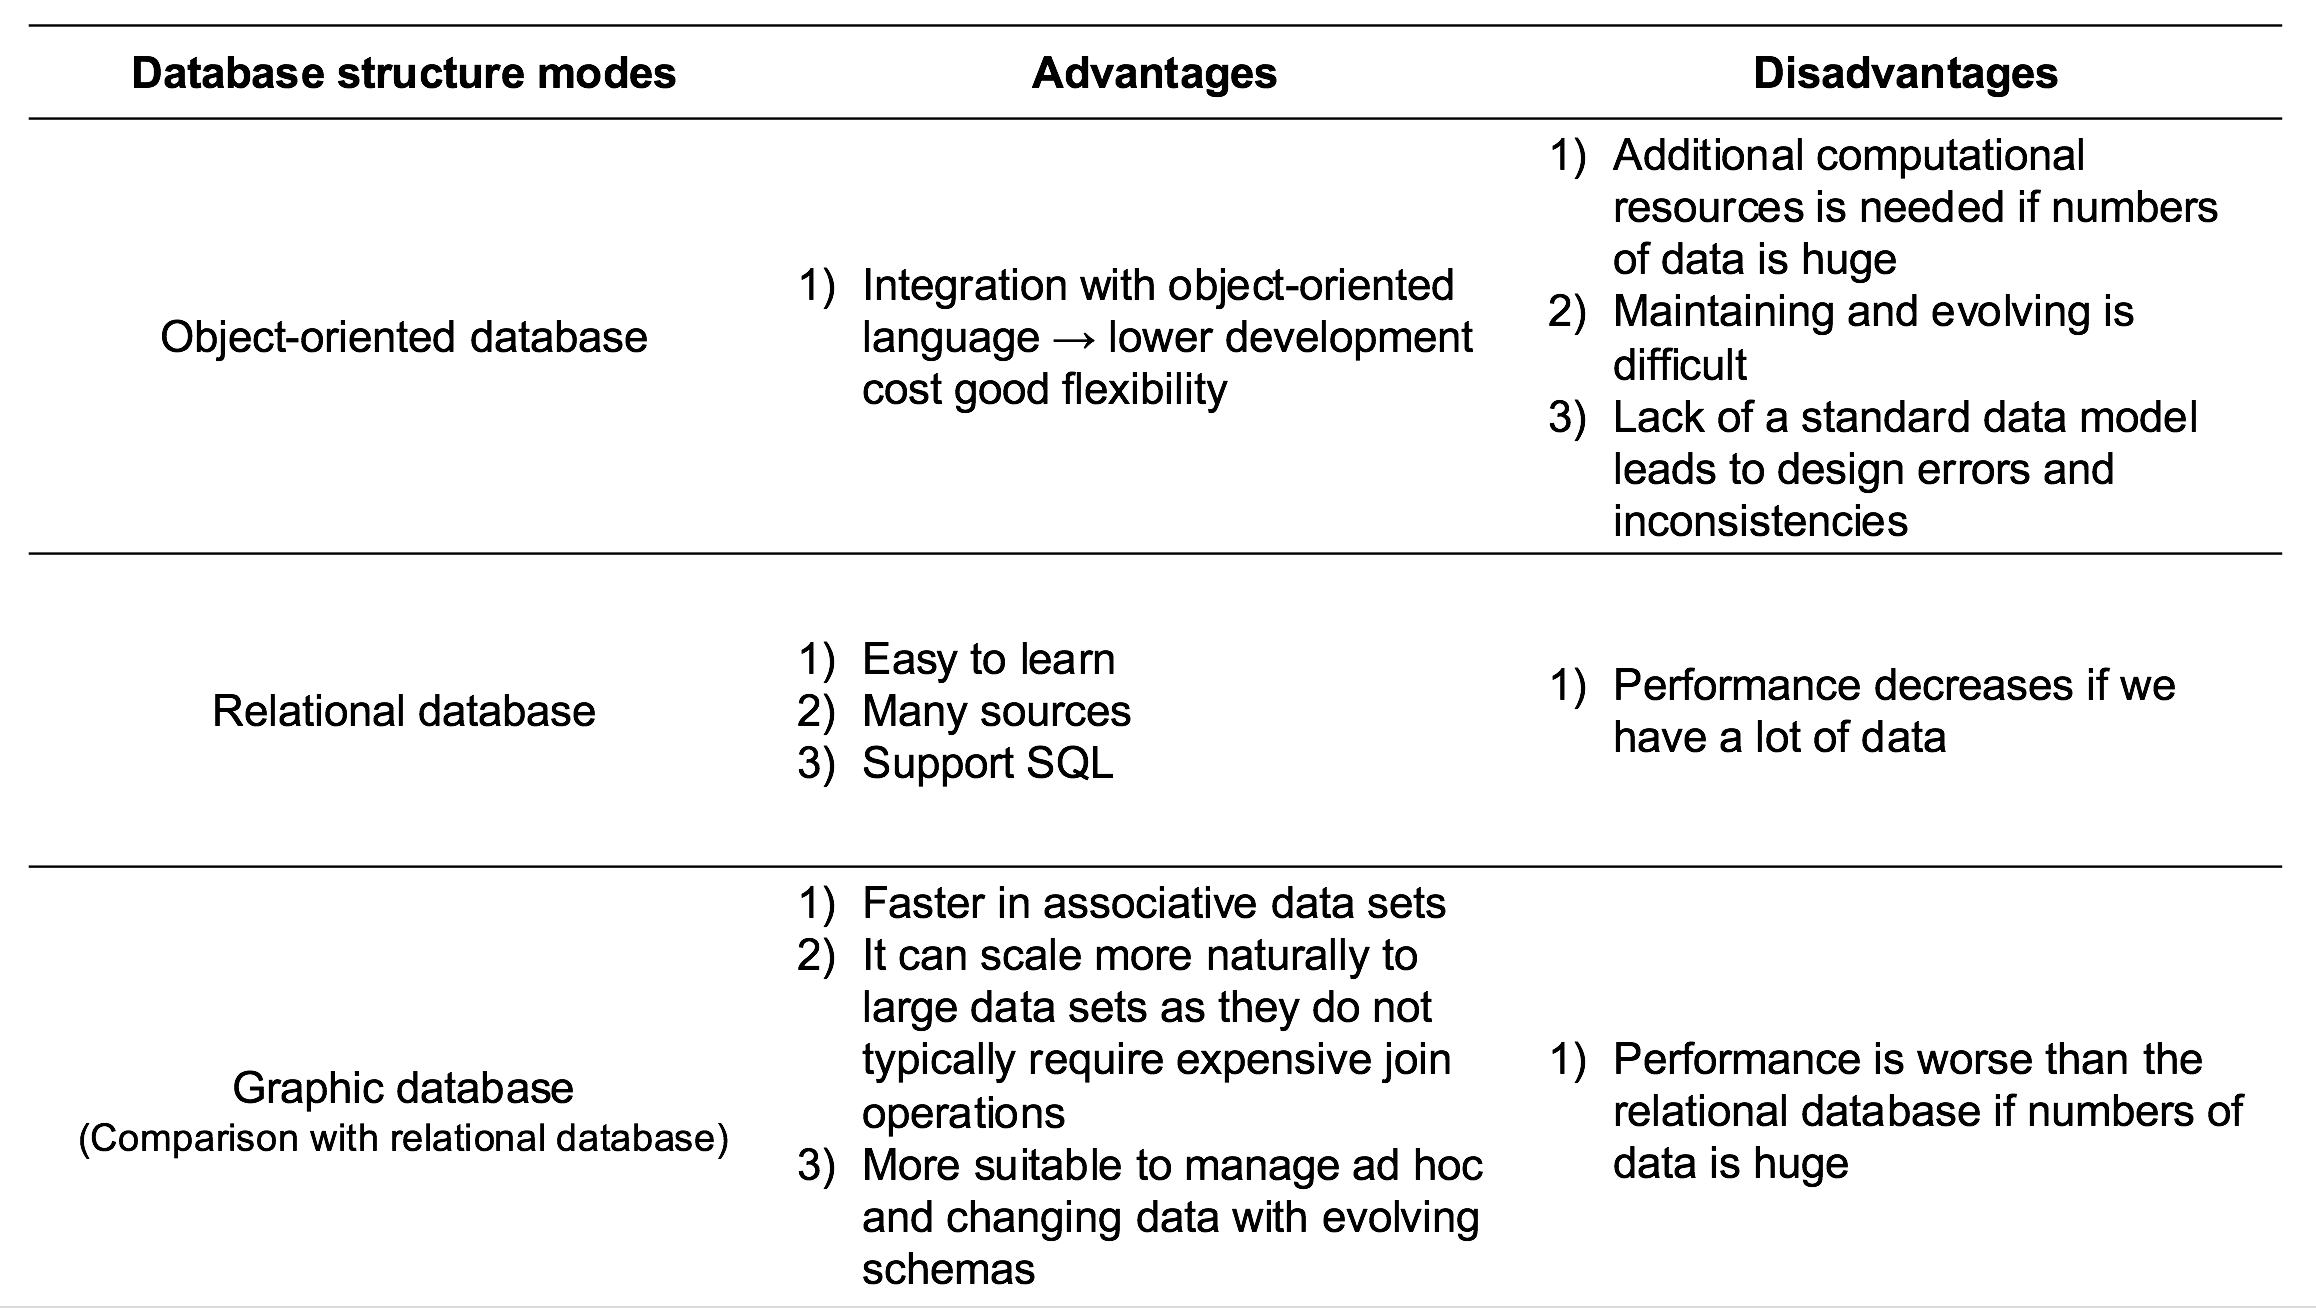
\includegraphics[width=1.8\columnwidth]{Wolverine_Method_Chart_2}
	\end{center}
	\caption{Advantages and disadvantages between three kind of databases.\label{WMC2}}	
\end{figure*}
\begin{figure*}[ht]
	\begin{center}
		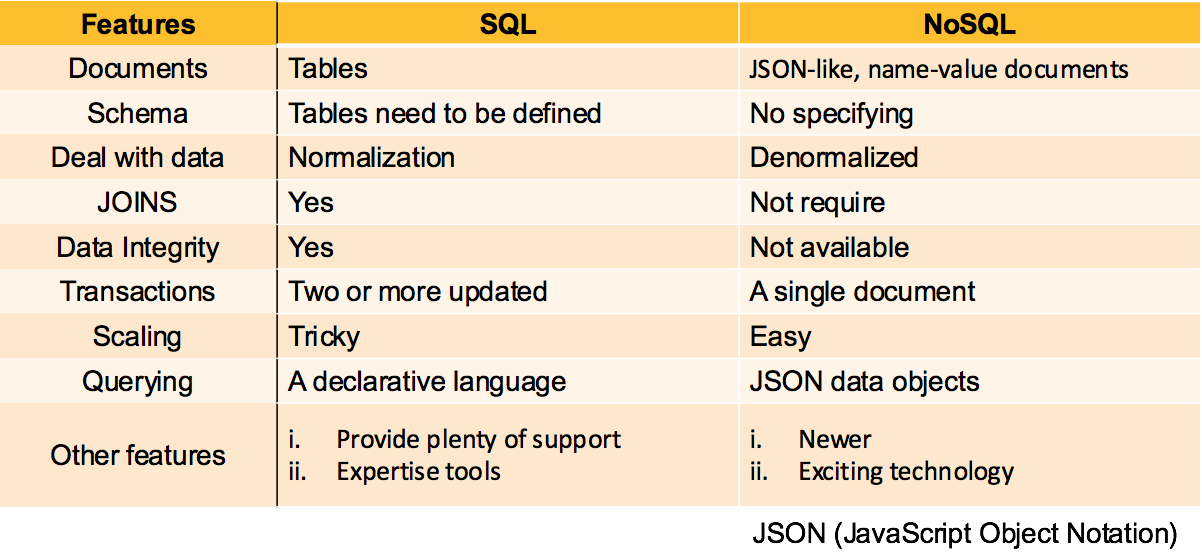
\includegraphics[width=1.8\columnwidth]{Wolverine_Method_Chart_3}
	\end{center}
	\caption{The differences between SQL and NoSQL. \label{WMC3}}
\end{figure*}

\newpage % Ends the current page and causes all figures and tables to be printed
